\documentclass[a4paper]{article}

\usepackage{graphicx}
\usepackage{amsmath,amssymb}
\usepackage{minted}
\usepackage{multirow}
\usepackage{float}
\usepackage{todonotes}
\usepackage{forest}
\usepackage{xstring}
\usepackage{xcolor}
\usepackage[most]{tcolorbox}
\usepackage{xparse}
\usepackage{natbib}

\usetikzlibrary{graphs,graphdrawing}
\usegdlibrary{layered}

% for external graphviz
\input{/home/donkarlo/Dropbox/repo/nd_language_ai_project/src/nd_language_ai/formal/computer/programming/tex/latex/code_clips/external_graphviz.tex}

% for tags
\input{/home/donkarlo/Dropbox/repo/nd_language_ai_project/src/nd_language_ai/formal/computer/programming/tex/latex/part/control_sequence/kind/semtag/semtag.tex}

% for links
\input{/home/donkarlo/Dropbox/repo/nd_language_ai_project/src/nd_language_ai/formal/computer/programming/tex/latex/code_clips/seehere.tex}

\title{Experiments}
\date{}
\author{Mohammad Rahmani}

\begin{document}
   \maketitle
   \begin{figure}[H]
      \centering
      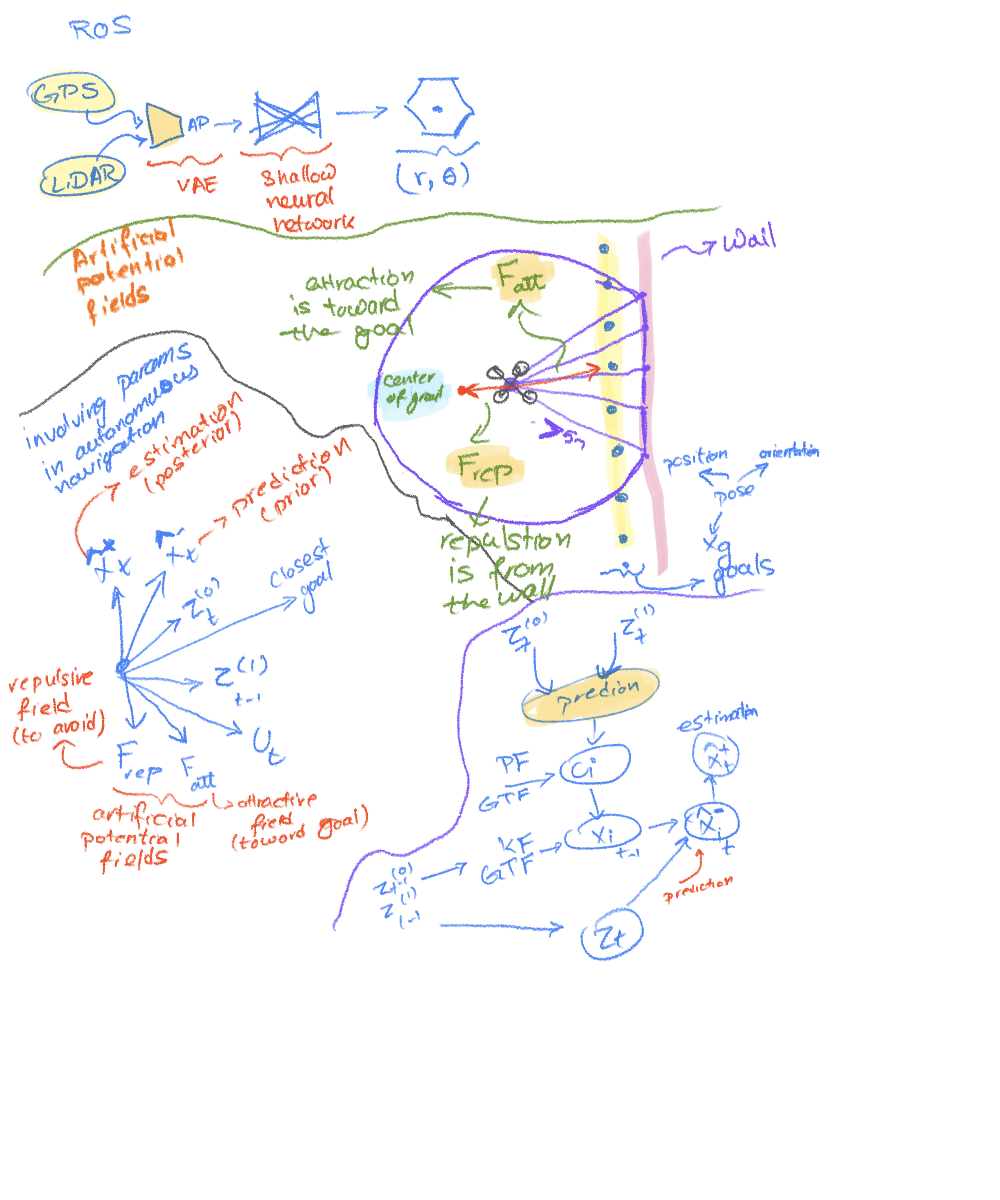
\includegraphics[width=0.9\textwidth]{artificial_field_potentials.png}
   \end{figure}
      \subsection{LiDAR scan polygon and its centroid}

         Consider a two-dimensional LiDAR that scans the complete \(360^\circ\) surrounding environment. Let \(N_{\mathrm{L}}\) denote the number of LiDAR rays in one complete scan. For the \(i\)-th ray, the LiDAR provides the scanning angle
         \[
         \phi_i^{\mathrm{L}}
         \]
         and the measured radial distance
         \[
         \rho_i^{\mathrm{L}},
         \qquad
         i=1,\ldots,N_{\mathrm{L}}.
         \]

         If a ray does not intersect an obstacle within the sensing range, a fixed maximum range is assigned to that ray. Therefore,
         \[
         \rho_i^{\mathrm{L}}
         =
         \begin{cases}
            \rho_{i,\mathrm{meas}}^{\mathrm{L}},
            & \text{if a valid return is obtained},\\[4pt]
            \rho_{\max}^{\mathrm{L}},
            & \text{otherwise},
         \end{cases}
         \]
         where, for example, \(\rho_{\max}^{\mathrm{L}}=5\,\mathrm{m}\).

         Each polar LiDAR measurement is transformed into a Cartesian point in the LiDAR coordinate frame as
         \[
         \mathbf{p}_i^{\mathrm{L}}
         =
         \begin{bmatrix}
            p_{x,i}^{\mathrm{L}}\\
            p_{y,i}^{\mathrm{L}}
         \end{bmatrix}
         =
         \begin{bmatrix}
            \rho_i^{\mathrm{L}}\cos\phi_i^{\mathrm{L}}\\
            \rho_i^{\mathrm{L}}\sin\phi_i^{\mathrm{L}}
         \end{bmatrix}.
         \]

         Because the measurements are ordered according to the scanning angle, consecutive points can be connected to form a closed polygon,
         \[
         \mathbf{p}_1^{\mathrm{L}}
         \rightarrow
         \mathbf{p}_2^{\mathrm{L}}
         \rightarrow
         \cdots
         \rightarrow
         \mathbf{p}_{N_{\mathrm{L}}}^{\mathrm{L}}
         \rightarrow
         \mathbf{p}_1^{\mathrm{L}}.
         \]

         For notational convenience, the polygon is closed by defining
         \[
         \mathbf{p}_{N_{\mathrm{L}}+1}^{\mathrm{L}}
         =
         \mathbf{p}_1^{\mathrm{L}}.
         \]

         The signed area of the resulting LiDAR polygon is
         \[
         \mathcal{A}_{\mathrm{L}}
         =
         \frac{1}{2}
         \sum_{i=1}^{N_{\mathrm{L}}}
         \left(
         p_{x,i}^{\mathrm{L}}p_{y,i+1}^{\mathrm{L}}
         -
         p_{x,i+1}^{\mathrm{L}}p_{y,i}^{\mathrm{L}}
         \right).
         \]

         Assuming a uniform density over the enclosed region, its geometric center of gravity, i.e.\ its area centroid, is defined as
         \[
         \mathbf{p}_{\mathrm{cg}}^{\mathrm{L}}
         =
         \begin{bmatrix}
            p_{\mathrm{cg},x}^{\mathrm{L}}\\
            p_{\mathrm{cg},y}^{\mathrm{L}}
         \end{bmatrix}.
         \]

         Its horizontal coordinate is
         \[
         p_{\mathrm{cg},x}^{\mathrm{L}}
         =
         \frac{1}{6\mathcal{A}_{\mathrm{L}}}
         \sum_{i=1}^{N_{\mathrm{L}}}
         \left(
         p_{x,i}^{\mathrm{L}}
         +
         p_{x,i+1}^{\mathrm{L}}
         \right)
         \left(
         p_{x,i}^{\mathrm{L}}p_{y,i+1}^{\mathrm{L}}
         -
         p_{x,i+1}^{\mathrm{L}}p_{y,i}^{\mathrm{L}}
         \right),
         \]
         and its vertical coordinate is
         \[
         p_{\mathrm{cg},y}^{\mathrm{L}}
         =
         \frac{1}{6\mathcal{A}_{\mathrm{L}}}
         \sum_{i=1}^{N_{\mathrm{L}}}
         \left(
         p_{y,i}^{\mathrm{L}}
         +
         p_{y,i+1}^{\mathrm{L}}
         \right)
         \left(
         p_{x,i}^{\mathrm{L}}p_{y,i+1}^{\mathrm{L}}
         -
         p_{x,i+1}^{\mathrm{L}}p_{y,i}^{\mathrm{L}}
         \right).
         \]

         This centroid is different from the arithmetic mean of the LiDAR endpoints,
         \[
         \frac{1}{N_{\mathrm{L}}}
         \sum_{i=1}^{N_{\mathrm{L}}}
         \mathbf{p}_i^{\mathrm{L}},
         \]
         because the latter represents only the mean position of the sampled boundary points, whereas
         \(\mathbf{p}_{\mathrm{cg}}^{\mathrm{L}}\) represents the centroid of the complete area enclosed by the scan polygon.

         When \(\rho_{\max}^{\mathrm{L}}\) is assigned to rays without a valid return, the resulting polygon represents the LiDAR-observable region truncated at the selected maximum range. Consequently,
         \(\mathbf{p}_{\mathrm{cg}}^{\mathrm{L}}\) is the centroid of this bounded LiDAR scan region and should not necessarily be interpreted as the geometric center of the complete physical environment.

         \input{/nd_research_publication/src/kind/journal_2026/experiments/comparative/comparative.tex}
         \input{/nd_research_publication/src/kind/journal_2026/experiments/simulation/simulation.tex}
         \input{/nd_research_publication/src/kind/journal_2026/experiments/code_implementation/code_implementation.tex}
         \bibliographystyle{plainnat}
         \bibliography{/home/donkarlo/Dropbox/repo/nd_shared_research/bibliography/bibliography.bib}
\end{document}